\chapter{Cristais I: o cristal perfeito e os metais}\label{ch:b1:crystals-metals}

Um fio de cobre pode ser estirado até ficar mais fino que um fio de
cabelo sem se romper; um torrão de sal se estilhaça sob uma martelada.
Um ferreiro aquece uma barra de ferro até ela brilhar, martela-a,
mergulha-a na água, e a barra sai muito mais dura do que entrou. A
diferença entre esses comportamentos está na maneira como os átomos se
empilham no sólido. A maioria dos sólidos são \omterm{def:b1:crystals-metals:crystal}{cristais}: seus átomos
ficam dispostos segundo um padrão que se repete, idêntico, bilhões de
vezes em todas as direções. Este capítulo descreve esses padrões, conta
seus átomos, mede o quão compactamente eles estão empilhados e onde
ficam os vazios entre eles, e usa o resultado para entender os metais e
as ligas. O próximo capítulo aplica as mesmas ferramentas aos sólidos
iônicos, covalentes e moleculares.

\begin{recall}
Os metais perdem facilmente seus \omterm{def:b1:quantum-numbers:configuration}{elétrons de valência}: têm baixas
energias de ionização e \omterm{def:b1:periodicity:electronegativity}{eletronegatividades} (\cref{ch:b1:periodicity}).
Os raios atômicos foram definidos na \cref{def:b1:periodicity:radius}. A
massa específica, propriedade estudada na física, é usada como
conhecida: $\rho = m/V$.
\end{recall}

\begin{omfigure}

\includegraphics[width=0.55\linewidth]{images/book2/ai/b1-05-blacksmith.jpg}

{\small Um ferreiro forjando aço. O ferro que brilha em laranja tem uma
estrutura cristalina diferente da do ferro à temperatura ambiente, e
pode reter mais carbono (problema de fim de semana).}
\end{omfigure}

\section{O modelo do cristal perfeito}

\begin{definition}[Cristal, sólido amorfo, cristal perfeito]\label{def:b1:crystals-metals:crystal}
Um \emph{cristal}\index{cristal} é um sólido cujas partículas (átomos,
íons ou moléculas) estão dispostas segundo um padrão que se repete
periodicamente nas três dimensões. Um sólido sem essa ordem de longo
alcance é um \emph{sólido amorfo}\index{solido amorfo@sólido amorfo} (o vidro, a maioria dos
plásticos). O \emph{modelo do cristal perfeito}\index{modelo do cristal perfeito} descreve um
cristal como infinito e sem defeitos: sem átomos faltando ou sobrando,
sem impurezas, sem contornos.
\end{definition}

\begin{definition}[Rede, motivo, célula unitária]\label{def:b1:crystals-metals:lattice}
Uma \emph{rede}\index{rede} é um conjunto infinito de pontos, os
\emph{nós}\index{no@nó}, obtidos a partir de um deles por todas as
translações $u\,\vec a + v\,\vec b + w\,\vec c$ com $u$, $v$,
$w$ inteiros. O \omterm{def:b1:crystals-metals:crystal}{cristal} é obtido colocando em cada nó o mesmo
\emph{motivo}\index{motivo} (um átomo, um grupo de átomos ou de íons).
Uma \emph{célula unitária}\index{celula unitaria@célula unitária} é um paralelepípedo construído sobre
$\vec a$, $\vec b$, $\vec c$ cujas translações preenchem o espaço; os
comprimentos de suas arestas e seus ângulos são os \emph{parâmetros de
rede}\index{parametros de rede@parâmetros de rede}
$a$, $b$, $c$, $\alpha$, $\beta$, $\gamma$. Em uma célula cúbica,
$a = b = c$ e os ângulos valem $90^\circ$.
\end{definition}

\begin{remark}[Cristais reais]\label{rem:b1:crystals-metals:real}
Os \omterm{def:b1:crystals-metals:crystal}{cristais} reais são finitos e imperfeitos: contêm lacunas, impurezas,
discordâncias e contornos de grão, que governam muitas propriedades (a
ductilidade do cobre, a dureza do aço). Esses defeitos são estudados no
volume do 3.º ano; o \omterm{def:b1:crystals-metals:crystal}{cristal} perfeito fornece a geometria, a massa
específica e a \omterm{def:b1:crystals-metals:compactness}{compacidade}, que os defeitos quase não alteram.
\end{remark}

\begin{definition}[Multiplicidade de uma célula]\label{def:b1:crystals-metals:multiplicity}
A \emph{multiplicidade}\index{multiplicidade} $Z$ de uma célula é o número de
\omterm{def:b1:crystals-metals:lattice}{motivos} (ou de átomos) que lhe pertencem, cada átomo compartilhado com
as células vizinhas contando pela fração que fica dentro dela.
\end{definition}

\begin{method}[Contar os átomos de uma célula]\label{met:b1:crystals-metals:count}
Em uma célula cúbica, um átomo em um vértice é compartilhado por 8
células e conta $1/8$; em uma aresta, é compartilhado por 4 e conta
$1/4$; em uma face, é compartilhado por 2 e conta $1/2$; no interior,
conta 1. Some as contribuições.
\end{method}

\begin{definition}[Número de coordenação]\label{def:b1:crystals-metals:coordination}
O \emph{número de coordenação}\index{numero de coordenacao@número de coordenação} de uma partícula
em um sólido é o número de seus vizinhos mais próximos, os que estão à
menor distância.
\end{definition}

\begin{definition}[Compacidade]\label{def:b1:crystals-metals:compactness}
A \emph{compacidade}\index{compacidade} (ou fator de empacotamento) de
um \omterm{def:b1:crystals-metals:crystal}{cristal} de esferas rígidas é a fração do volume ocupada pelas
esferas: para uma célula de volume $V$ que contém $Z$ esferas de raio $R$,
\[
  C = \frac{Z \cdot \frac43 \pi R^3}{V} .
\]
\end{definition}

\begin{proposition}[Massa específica a partir da célula]\label{prop:b1:crystals-metals:density}
A massa específica de um \omterm{def:b1:crystals-metals:crystal}{cristal} cuja célula, de volume $V$, contém $Z$
partículas de massa molar $M$ é
\[
  \rho = \frac{Z\,M}{N_A\,V} .
\]
\end{proposition}

\begin{proof}
A célula contém $Z$ partículas, de massa $Z\,M/N_A$; o \omterm{def:b1:crystals-metals:crystal}{cristal} é a
célula repetida, de modo que sua massa específica é a de uma célula.
\end{proof}

\section{Empacotamentos compactos: cúbico de faces centradas e hexagonal}

\begin{definition}[Empacotamento compacto, CFC, HC]\label{def:b1:crystals-metals:packings}
Um \emph{empacotamento compacto}\index{empacotamento compacto} de esferas idênticas é
construído a partir de camadas compactas, em que cada esfera toca outras
seis, empilhadas de modo que cada esfera de uma camada fique em uma
cavidade da camada de baixo. O empilhamento $ABCABC\dots$ dá a estrutura
\emph{cúbica de faces centradas}\index{cubica de faces centradas@cúbica de faces centradas}
(CFC, ou cúbica compacta); o empilhamento $ABAB\dots$
dá a estrutura \emph{hexagonal compacta}\index{hexagonal compacta}
(HC). Uma terceira estrutura dos metais, não compacta, é a estrutura
\emph{cúbica de corpo centrado}\index{cubica de corpo centrado@cúbica de corpo centrado} (CCC), um
cubo com um átomo em cada vértice e um em seu centro.
\end{definition}

\begin{omfigure}
\begin{tikzpicture}[font=\small]
  % layer A
  \foreach \i in {0,...,4} \foreach \j in {0,...,3} {
    \pgfmathsetmacro\x{\i+0.5*\j}
    \pgfmathsetmacro\y{0.866*\j}
    \draw[black!60, fill=omDef!25] (\x,\y) circle (0.5);
  }
  % layer B, in the hollows pointing up
  \foreach \i/\j in {1/0, 2/0, 3/0, 1/1, 2/1, 3/1, 1/2, 2/2} {
    \pgfmathsetmacro\x{\i+0.5*\j}
    \pgfmathsetmacro\y{0.866*\j+0.577}
    \draw[omThm!80!black, fill=omThm!25, fill opacity=0.75] (\x,\y) circle (0.5);
  }
  % C positions
  \foreach \i/\j in {1/0, 2/0, 3/0, 1/1, 2/1, 3/1} {
    \pgfmathsetmacro\x{\i+0.5+0.5*\j}
    \pgfmathsetmacro\y{0.866*\j+0.289}
    \fill[omMeth] (\x,\y) circle (0.11);
  }
  \node[anchor=west, align=left] at (6.6,1.6) {A: primeira camada (azul)\\B: segunda camada, nas\\\phantom{B: }cavidades de A (vermelho)\\C: as outras cavidades\\\phantom{C: }(pontos verdes)};
\end{tikzpicture}

{\small Duas camadas compactas vistas de cima. Uma terceira camada pode
ficar acima das cavidades marcadas C (empilhamento $ABC$, \omterm{def:b1:crystals-metals:packings}{cúbico de
faces centradas}) ou acima dos átomos de A (empilhamento $AB$, \omterm{def:b1:crystals-metals:packings}{hexagonal
compacto}).}
\end{omfigure}

\begin{proposition}[Cúbica de faces centradas]\label{prop:b1:crystals-metals:fcc}
Na estrutura CFC, os átomos ocupam os oito vértices e os seis centros
das faces de um cubo de aresta $a$. Então $Z = 4$, o \omterm{def:b1:crystals-metals:coordination}{número de
coordenação} é 12, os átomos se tocam ao longo de uma diagonal de face,
$a\sqrt2 = 4R$, e a \omterm{def:b1:crystals-metals:compactness}{compacidade} é
\[
  C = \frac{\pi}{3\sqrt2} \approx 0.74 .
\]
\end{proposition}

\begin{proof}
$Z = 8 \times \frac18 + 6 \times \frac12 = 4$. Um átomo no centro de uma
face toca os quatro vértices de sua face e os quatro centros de face de
cada uma das duas células que compartilham a face: $4 + 4 + 4 = 12$
vizinhos a $a\sqrt2/2$. Em uma diagonal de face, de comprimento $a\sqrt2$,
ficam um átomo de vértice, um átomo de centro de face e um átomo de
vértice em contato: $a\sqrt2 = 4R$. Então
$C = 4 \cdot \frac43\pi R^3/a^3 = \frac{16}{3}\pi R^3/(2\sqrt2 R)^3 \cdot
\frac{1}{1} = \frac{16\pi}{3 \times 16\sqrt2} = \frac{\pi}{3\sqrt2}$.
\end{proof}

\begin{omfigure}
\tdplotsetmaincoords{60}{100}
\begin{tikzpicture}[tdplot_main_coords, font=\small]
  \pic {omcubeo={3}};
  \node[cellA=6mm] at (0,0,0) {};
  \node[cellA=6mm] at (0,3,0) {};
  \node[cellA=6mm, ball color=omDef!55] at (0,1.5,1.5) {};
  \node[cellA=6mm] at (0,0,3) {};
  \node[cellA=6mm, ball color=omDef!55] at (1.5,1.5,0) {};
  \node[cellA=6mm] at (0,3,3) {};
  \node[cellA=6mm, ball color=omDef!55] at (1.5,0,1.5) {};
  \node[cellA=6mm, ball color=omDef!55] at (1.5,3,1.5) {};
  \node[cellA=6mm] at (3,0,0) {};
  \node[cellA=6mm, ball color=omDef!55] at (1.5,1.5,3) {};
  \node[cellA=6mm] at (3,3,0) {};
  \node[cellA=6mm, ball color=omDef!55] at (3,1.5,1.5) {};
  \node[cellA=6mm] at (3,0,3) {};
  \node[cellA=6mm] at (3,3,3) {};
  \draw[omThm, thick] (3,0,0) -- (3,3,3);
\end{tikzpicture}
\hspace{1.2cm}
\begin{tikzpicture}[tdplot_main_coords, font=\small]
  \pic {omcubeo={3}};
  \node[cellA=7mm] at (0,0,0) {};
  \node[cellA=7mm] at (0,3,0) {};
  \node[cellA=7mm] at (0,0,3) {};
  \node[cellA=7mm] at (0,3,3) {};
  \node[cellA=7mm, ball color=omDef!55] at (1.5,1.5,1.5) {};
  \node[cellA=7mm] at (3,0,0) {};
  \node[cellA=7mm] at (3,3,0) {};
  \node[cellA=7mm] at (3,0,3) {};
  \node[cellA=7mm] at (3,3,3) {};
  \draw[omThm, thick] (3,0,0) -- (0,3,3);
\end{tikzpicture}

{\small À esquerda: a célula \omterm{def:b1:crystals-metals:packings}{cúbica de faces centradas} (átomos dos
vértices em cinza, átomos dos centros das faces em azul). Os átomos se
tocam ao longo de uma diagonal de face (linha vermelha,
$a\sqrt2 = 4R$). À direita: a célula \omterm{def:b1:crystals-metals:packings}{cúbica de corpo centrado}; os átomos
se tocam ao longo da diagonal principal (linha vermelha, $a\sqrt3 = 4R$).
Átomos desenhados menores que o tamanho de contato, para maior clareza.}
\end{omfigure}

\begin{proposition}[Hexagonal compacta]\label{prop:b1:crystals-metals:hcp}
Na estrutura HC, o prisma hexagonal convencional, de aresta da base $a$
e altura $c$, contém 6 átomos; o \omterm{def:b1:crystals-metals:coordination}{número de coordenação} é 12; para
esferas em contato, $a = 2R$, $c/a = \sqrt{8/3} \approx 1.633$, e a
\omterm{def:b1:crystals-metals:compactness}{compacidade} é a mesma da CFC, $\pi/(3\sqrt2) \approx 0.74$.
\end{proposition}

\begin{proof}
O prisma tem 12 átomos de vértice compartilhados por 6 prismas, 2 átomos
de centro de face compartilhados por 2 e 3 átomos internos:
$12/6 + 2/2 + 3 = 6$. Cada átomo toca seis vizinhos em sua camada e três
em cada camada adjacente: 12. Um átomo da camada B fica sobre três
átomos em contato da camada A, formando um tetraedro regular de aresta
$2R$, cuja altura é $2R\sqrt{2/3}$; duas camadas acima,
$c = 4R\sqrt{2/3}$, de modo que $c/a = 2\sqrt{2/3} = \sqrt{8/3}$. O volume
do prisma é $\frac{3\sqrt3}{2}a^2 c = \frac{3\sqrt3}{2}(2R)^2 \cdot
4R\sqrt{2/3} = 24\sqrt2\,R^3$, e $C = 6 \cdot \frac43\pi R^3/(24\sqrt2
R^3) = \pi/(3\sqrt2)$.
\end{proof}

\begin{omfigure}
\tdplotsetmaincoords{70}{113}
\begin{tikzpicture}[tdplot_main_coords, font=\small, scale=1.25]
  \pic[transform shape] {omhexprismo={1.6}{2.6}};
  \node[cellA=6mm] at (-1.6,0,0) {};
  \node[cellA=6mm] at (-0.8,-1.386,0) {};
  \node[cellA=6mm] at (-1.6,0,2.6) {};
  \node[cellA=6mm] at (-0.8,-1.386,2.6) {};
  \node[cellA=6mm] at (-0.8,1.386,0) {};
  \node[cellA=6mm, ball color=omThm!60] at (-0.8,0.462,1.3) {};
  \node[cellA=6mm] at (0,0,0) {};
  \node[cellA=6mm, ball color=omThm!60] at (0,-0.924,1.3) {};
  \node[cellA=6mm] at (0.8,-1.386,0) {};
  \node[cellA=6mm] at (-0.8,1.386,2.6) {};
  \node[cellA=6mm] at (0,0,2.6) {};
  \node[cellA=6mm] at (0.8,-1.386,2.6) {};
  \node[cellA=6mm] at (0.8,1.386,0) {};
  \node[cellA=6mm, ball color=omThm!60] at (0.8,0.462,1.3) {};
  \node[cellA=6mm] at (1.6,0,0) {};
  \node[cellA=6mm] at (0.8,1.386,2.6) {};
  \node[cellA=6mm] at (1.6,0,2.6) {};
\end{tikzpicture}

{\small O prisma \omterm{def:b1:crystals-metals:packings}{hexagonal compacto}, de aresta da base $a$ (o lado do
hexágono) e altura $c$: camadas A (cinza) na base e no topo, camada B
(vermelho) a meia altura, assentada nas cavidades de A.}
\end{omfigure}

\section{Cúbica de corpo centrado e os elementos metálicos}

\begin{proposition}[Cúbica de corpo centrado]\label{prop:b1:crystals-metals:bcc}
Na estrutura CCC, $Z = 2$, o \omterm{def:b1:crystals-metals:coordination}{número de coordenação} é 8, os átomos se
tocam ao longo da diagonal principal do cubo, $a\sqrt3 = 4R$, e a
\omterm{def:b1:crystals-metals:compactness}{compacidade} é
\[
  C = \frac{\pi\sqrt3}{8} \approx 0.68 .
\]
\end{proposition}

\begin{proof}
$Z = 8 \times \frac18 + 1 = 2$. O átomo central toca os oito vértices: a
diagonal principal $a\sqrt3$ contém um vértice, o centro e um vértice,
$a\sqrt3 = 4R$. Então $C = 2 \cdot \frac43\pi R^3/a^3 =
\frac83\pi R^3 (\sqrt3/(4R))^3 = \frac83\pi \cdot \frac{3\sqrt3}{64} =
\frac{\pi\sqrt3}{8}$.
\end{proof}

\begin{proposition}[O empacotamento compacto é o mais denso]\label{prop:b1:crystals-metals:kepler}
Nenhum empacotamento de esferas idênticas tem \omterm{def:b1:crystals-metals:compactness}{compacidade} maior que
$\pi/(3\sqrt2) \approx 0.7405$, o valor da CFC e da HC.
\end{proposition}
\admitted

\begin{history}[A conjectura de Kepler, 1611--2017]
Em um breve ensaio sobre os flocos de neve, escrito em 1611, Johannes
Kepler afirmou que nenhuma maneira de empilhar balas de canhão podia ser
mais densa que a pirâmide do quitandeiro, o empacotamento \omterm{def:b1:crystals-metals:packings}{cúbico de faces
centradas}. A afirmação resistiu à demonstração por quase quatro séculos.
Thomas Hales deu uma demonstração assistida por computador em 1998, e uma
demonstração formal, verificada linha por linha por computador, foi
concluída em 2014 e publicada em 2017.
\end{history}

\begin{example}[Três metais]\label{ex:b1:crystals-metals:metals}
O cobre é CFC com $a = \qty{361.5}{pm}$: $R = a\sqrt2/4 =
\qty{127.8}{pm}$ e $\rho = 4 \times 63.55/(6.022 \times 10^{23} \times
(3.615 \times 10^{-8})^3) = \qty{8.93}{g/cm^3}$, a massa específica medida.
O ferro à temperatura ambiente (ferro $\alpha$) é CCC com $a = \qty{286.7}{pm}$:
$R = \qty{124.1}{pm}$, $\rho = \qty{7.87}{g/cm^3}$. O magnésio é HC com
$a = \qty{320.9}{pm}$ e $c = \qty{521.0}{pm}$: $c/a = 1.624$, próximo do
valor ideal $1.633$; o zinco, com $c/a = 1.856$, é um empacotamento
hexagonal alongado.
% ledger: lat:Cu, rho:Cu, lat:Fe-alpha, rho:Fe, lat:Mg.a, lat:Mg.c,
% lat:Zn.a, lat:Zn.c, aw:Cu, aw:Fe, const:NA
\end{example}

\begin{center}
\small
\begin{tabular}{lllccc}
\hline
metal & estrutura & $a$ (pm) & $R$ (pm) & $\rho$ calculada & $\rho$ medida \\
\hline
alumínio & CFC & 405.0 & 143.2 & 2.70 & 2.70 \\
cobre & CFC & 361.5 & 127.8 & 8.93 & 8.93 \\
prata & CFC & 408.6 & 144.5 & 10.50 & 10.50 \\
sódio & CCC & 429.1 & 185.8 & 0.967 & 0.97 \\
ferro $\alpha$ & CCC & 286.7 & 124.1 & 7.87 & 7.87 \\
tungstênio & CCC & 316.5 & 137.0 & 19.26 & 19.3 \\
\hline
\end{tabular}
\end{center}
% ledger: lat:Al, lat:Cu, lat:Ag, lat:Na, lat:Fe-alpha, lat:W, rho:Al,
% rho:Cu, rho:Ag, rho:Na, rho:Fe, rho:W (densities in g/cm3)

\begin{omfigure}
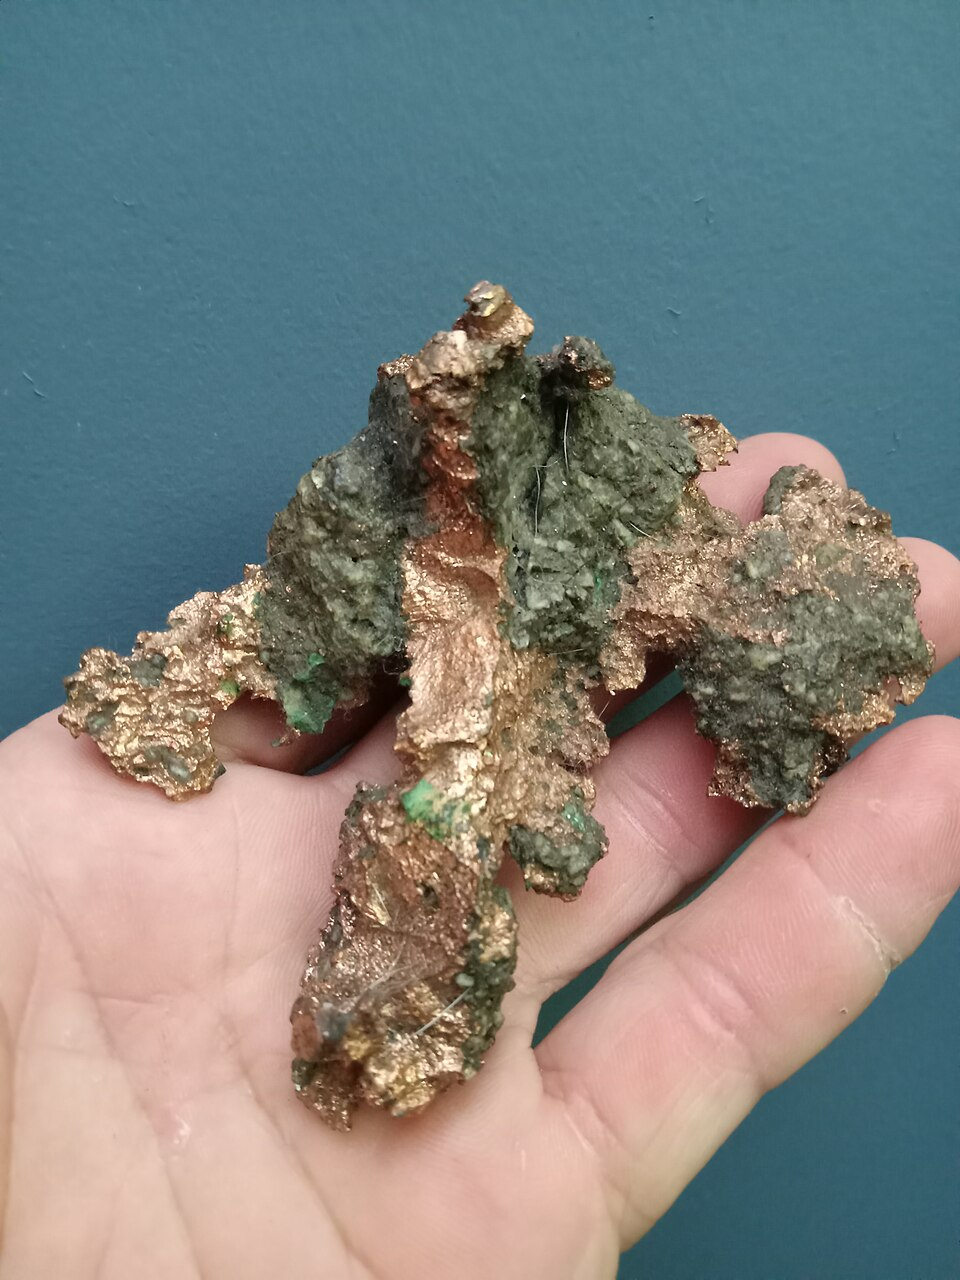
\includegraphics[width=0.36\linewidth]{images/book2/native-copper.jpg}

{\small Uma amostra de cobre nativo. Suas formas ramificadas cresceram
como \omterm{def:b1:crystals-metals:crystal}{cristais}; o metal por baixo é um mosaico de grãos CFC.
Foto: CC0 (Wikimedia Commons).}
\end{omfigure}

\section{Sítios intersticiais}

\begin{definition}[Sítios intersticiais]\label{def:b1:crystals-metals:site}
Um \emph{sítio intersticial}\index{sitio intersticial@sítio intersticial} é um vazio entre os
átomos de um \omterm{def:b1:crystals-metals:crystal}{cristal} onde um átomo menor pode se alojar. Um \emph{sítio
tetraédrico}\index{sitio tetraedrico@sítio tetraédrico} fica no centro de um tetraedro de quatro
átomos; um \emph{sítio octaédrico}\index{sitio octaedrico@sítio octaédrico}, no centro de um
octaedro de seis. A \emph{habitabilidade}\index{habitabilidade} de um
sítio é o raio da maior esfera que cabe nele sem afastar os átomos
vizinhos.
\end{definition}

\begin{proposition}[Sítios da estrutura CFC]\label{prop:b1:crystals-metals:sites}
Uma célula CFC contém 4 \omterm{def:b1:crystals-metals:site}{sítios octaédricos}, no centro do cubo e nos
pontos médios de suas 12 arestas, e 8 \omterm{def:b1:crystals-metals:site}{sítios tetraédricos}, nos centros
dos 8 cubinhos de aresta $a/2$. Para átomos de raio $R$ em contato, as
\omterm{def:b1:crystals-metals:site}{habitabilidades} são
\[
  r_O = (\sqrt2 - 1)R \approx 0.414\,R, \qquad
  r_T = \left(\sqrt{\tfrac32} - 1\right)R \approx 0.225\,R .
\]
\end{proposition}

\begin{proof}
\omterm{def:b1:crystals-metals:site}{Sítios octaédricos}: $1 + 12 \times \frac14 = 4$, tantos quanto átomos. O
centro do cubo está a $a/2$ dos seis centros de face: $r_O + R = a/2$
com $a = 2\sqrt2 R$, logo $r_O = (\sqrt2 - 1)R$. \omterm{def:b1:crystals-metals:site}{Sítios tetraédricos}: o
centro de um cubinho de aresta $a/2$ fica à metade de sua diagonal
principal,
$\frac{a}{2}\cdot\frac{\sqrt3}{2} = \frac{a\sqrt3}{4}$, dos quatro
átomos situados em vértices alternados: $r_T + R = \frac{\sqrt3}{4}\,2\sqrt2\,R =
\sqrt{\tfrac32}\,R$.
\end{proof}

\begin{omfigure}
\tdplotsetmaincoords{60}{100}
\begin{tikzpicture}[tdplot_main_coords, font=\small]
  \pic {omcubeo={3}};
  \node[cellA=3.6mm] at (0,0,0) {};
  \node[cellsite=4mm, draw=omThm, fill=omThm!30] at (0,1.5,0) {};
  \node[cellA=3.6mm] at (0,3,0) {};
  \node[cellsite=4mm, draw=omThm, fill=omThm!30] at (0,0,1.5) {};
  \node[cellA=3.6mm] at (0,1.5,1.5) {};
  \node[cellsite=4mm, draw=omThm, fill=omThm!30] at (0,3,1.5) {};
  \node[cellsite=4mm, draw=omThm, fill=omThm!30] at (1.5,0,0) {};
  \node[cellA=3.6mm] at (0,0,3) {};
  \node[cellA=3.6mm] at (1.5,1.5,0) {};
  \node[cellsite=4mm, draw=omThm, fill=omThm!30] at (0,1.5,3) {};
  \node[cellsite=4mm, draw=omThm, fill=omThm!30] at (1.5,3,0) {};
  \node[cellA=3.6mm] at (0,3,3) {};
  \node[cellA=3.6mm] at (1.5,0,1.5) {};
  \node[cellsite=5mm, draw=omThm, fill=omThm!30] at (1.5,1.5,1.5) {};
  \node[cellA=3.6mm] at (1.5,3,1.5) {};
  \node[cellA=3.6mm] at (3,0,0) {};
  \node[cellsite=4mm, draw=omThm, fill=omThm!30] at (1.5,0,3) {};
  \node[cellsite=4mm, draw=omThm, fill=omThm!30] at (3,1.5,0) {};
  \node[cellA=3.6mm] at (1.5,1.5,3) {};
  \node[cellA=3.6mm] at (3,3,0) {};
  \node[cellsite=4mm, draw=omThm, fill=omThm!30] at (1.5,3,3) {};
  \node[cellsite=4mm, draw=omThm, fill=omThm!30] at (3,0,1.5) {};
  \node[cellA=3.6mm] at (3,1.5,1.5) {};
  \node[cellsite=4mm, draw=omThm, fill=omThm!30] at (3,3,1.5) {};
  \node[cellA=3.6mm] at (3,0,3) {};
  \node[cellsite=4mm, draw=omThm, fill=omThm!30] at (3,1.5,3) {};
  \node[cellA=3.6mm] at (3,3,3) {};
  \node[below] at (1.5,1.5,-1.5) {sítios octaédricos (vermelho)};
\end{tikzpicture}
\hspace{1.2cm}
\begin{tikzpicture}[tdplot_main_coords, font=\small]
  \pic {omcubeo={3}};
  \node[cellA=3.6mm] at (0,0,0) {};
  \node[cellA=3.6mm] at (0,3,0) {};
  \node[cellA=3.6mm] at (0,1.5,1.5) {};
  \node[cellsite=4mm, fill=omDef!30] at (0.75,0.75,0.75) {};
  \node[cellsite=4mm, fill=omDef!30] at (0.75,2.25,0.75) {};
  \node[cellA=3.6mm] at (0,0,3) {};
  \node[cellA=3.6mm] at (1.5,1.5,0) {};
  \node[cellsite=4mm, fill=omDef!30] at (0.75,0.75,2.25) {};
  \node[cellA=3.6mm] at (0,3,3) {};
  \node[cellA=3.6mm] at (1.5,0,1.5) {};
  \node[cellsite=4mm, fill=omDef!30] at (0.75,2.25,2.25) {};
  \node[cellsite=4mm, fill=omDef!30] at (2.25,0.75,0.75) {};
  \node[cellA=3.6mm] at (1.5,3,1.5) {};
  \node[cellA=3.6mm] at (3,0,0) {};
  \node[cellsite=4mm, fill=omDef!30] at (2.25,2.25,0.75) {};
  \node[cellA=3.6mm] at (1.5,1.5,3) {};
  \node[cellA=3.6mm] at (3,3,0) {};
  \node[cellsite=4mm, fill=omDef!30] at (2.25,0.75,2.25) {};
  \node[cellsite=4mm, fill=omDef!30] at (2.25,2.25,2.25) {};
  \node[cellA=3.6mm] at (3,1.5,1.5) {};
  \node[cellA=3.6mm] at (3,0,3) {};
  \node[cellA=3.6mm] at (3,3,3) {};
  \draw[omDef!70!black, thin] (0,0,0) -- (0.75,0.75,0.75) -- (1.5,1.5,0)
    (0.75,0.75,0.75) -- (1.5,0,1.5) (0.75,0.75,0.75) -- (0,1.5,1.5);
  \node[below] at (1.5,1.5,-1.5) {sítios tetraédricos (azul)};
\end{tikzpicture}

{\small \omterm{def:b1:crystals-metals:site}{Sítios intersticiais} da célula CFC. À esquerda: o \omterm{def:b1:crystals-metals:site}{sítio
octaédrico} do centro e os dos pontos médios das arestas (compartilhados
por quatro células). À direita: os oito \omterm{def:b1:crystals-metals:site}{sítios tetraédricos} nos centros
dos oitavos do cubo, um deles ligado a seus quatro átomos.}
\end{omfigure}

\section{Ligação metálica e ligas}

\begin{definition}[Ligação metálica]\label{def:b1:crystals-metals:metallic-bond}
Na \emph{ligação metálica}\index{ligacao metalica@ligação metálica}, cada átomo de um metal
cede seus \omterm{def:b1:quantum-numbers:configuration}{elétrons de valência} ao \omterm{def:b1:crystals-metals:crystal}{cristal} inteiro: o sólido é uma \omterm{def:b1:crystals-metals:lattice}{rede}
de cátions banhados por elétrons que não pertencem a nenhum átomo em
particular e se movem livremente por ele. A ligação é a atração entre os
cátions e essa nuvem eletrônica compartilhada; ela não é direcional.
\end{definition}

\begin{proposition}[Propriedades dos metais]\label{prop:b1:crystals-metals:properties}
A \omterm{def:b1:crystals-metals:metallic-bond}{ligação metálica} explica as propriedades dos metais: os elétrons
móveis conduzem eletricidade e calor e refletem a luz (o brilho); como a
ligação não é direcional, camadas de átomos podem deslizar umas sobre as
outras sem romper o \omterm{def:b1:crystals-metals:crystal}{cristal} (ductilidade, maleabilidade), e os
\omterm{def:b1:crystals-metals:packings}{empacotamentos compactos}, que maximizam o número de vizinhos, são as
estruturas mais comuns.
\end{proposition}
\admitted

\begin{definition}[Ligas]\label{def:b1:crystals-metals:alloy}
Uma liga é um sólido metálico formado por vários elementos. Em uma
\emph{liga de substituição}\index{liga de substituicao@liga de substituição}, os átomos do
elemento adicionado substituem átomos do hospedeiro em sua \omterm{def:b1:crystals-metals:lattice}{rede}; isso
exige raios que não difiram mais de cerca de 15\,\% (cobre e níquel,
cobre e zinco no latão). Em uma \emph{liga intersticial}\index{liga intersticial},
átomos pequenos (\ce{H}, \ce{C}, \ce{N}, \ce{B}) ocupam \omterm{def:b1:crystals-metals:site}{sítios
intersticiais} do hospedeiro (o carbono no aço).
\end{definition}

\begin{definition}[Alotropia]\label{def:b1:crystals-metals:allotropy}
As diferentes estruturas cristalinas de um mesmo elemento são seus
\emph{alótropos}\index{alotropo@alótropo}. O ferro é CCC (ferro $\alpha$) à temperatura
ambiente; as medidas o mostram CFC (ferro $\gamma$) de \qty{1189}{K} a
\qty{1661}{K}, e de novo CCC (ferro $\delta$) a \qty{1662}{K}, até seu
ponto de fusão. O carbono existe como diamante e como grafite
(\cref{ch:b1:crystals-ionic-covalent}).
% ledger: lat:Fe-alpha, lat:Fe-gamma-1189, lat:Fe-gamma-1661,
% lat:Fe-delta-1662
\end{definition}

\begin{example}[O aço]\label{ex:b1:crystals-metals:steel}
O carbono, de \omterm{def:b1:periodicity:radius}{raio covalente} \qty{77}{pm} (metade da distância \ce{C-C}
no diamante), é grande demais para os sítios do ferro sem distorção, mas
muito menos no ferro $\gamma$, cujos \omterm{def:b1:crystals-metals:site}{sítios octaédricos} são os maiores. O
aço é feito dissolvendo carbono no ferro $\gamma$ quente; com a têmpera,
o carbono fica preso enquanto o ferro volta a uma estrutura de corpo
centrado, que ele distorce, e o \omterm{def:b1:crystals-metals:crystal}{cristal} distorcido é duro.
% ledger: lat:C-diamond (r = a sqrt3 / 8 = 77.2 pm)
\end{example}

\begin{remark}[As transições do ferro]\label{rem:b1:crystals-metals:iron-T}
As temperaturas da \cref{def:b1:crystals-metals:allotropy} são as do
ferro puro à pressão atmosférica; o carbono dissolvido abaixa a
temperatura em que se forma o ferro $\gamma$, o que torna o aço
trabalhável. Os diagramas de fases das ligas são estudados no volume do
2.º ano.
\end{remark}

\section{Exercícios}

\begin{exercise}[$\star$]\label{exo:b1:crystals-metals:1}
Conte os átomos de uma célula cúbica simples (átomos apenas nos
vértices), de uma célula CCC e de uma célula CFC, e dê o \omterm{def:b1:crystals-metals:coordination}{número de
coordenação} em cada caso.
\end{exercise}

\begin{exercise}[$\star$]\label{exo:b1:crystals-metals:2}
Mostre que a \omterm{def:b1:crystals-metals:compactness}{compacidade} da estrutura cúbica simples (átomos em contato
ao longo de uma aresta) é $\pi/6$, e compare com a CFC e a CCC.
\end{exercise}

\begin{exercise}[$\star$]\label{exo:b1:crystals-metals:3}
O alumínio é CFC com $a = \qty{405.0}{pm}$. Calcule seu raio atômico e
sua massa específica ($M = \qty{26.98}{g/mol}$).
% ledger: lat:Al, aw:Al
\end{exercise}

\begin{exercise}[$\star$]\label{exo:b1:crystals-metals:4}
O sódio é CCC com $a = \qty{429.1}{pm}$. Calcule seu raio atômico e
sua massa específica ($M = \qty{22.99}{g/mol}$), e compare com o valor
medido, \qty{0.97}{g/cm^3}.
% ledger: lat:Na, rho:Na, aw:Na
\end{exercise}

\begin{exercise}[$\star\star$]\label{exo:b1:crystals-metals:5}
A prata é CFC e sua massa específica é \qty{10.50}{g/cm^3}
($M = \qty{107.87}{g/mol}$). Calcule o \omterm{def:b1:crystals-metals:lattice}{parâmetro de rede} e o raio
atômico.
% ledger: rho:Ag, aw:Ag
\end{exercise}

\begin{exercise}[$\star\star$]\label{exo:b1:crystals-metals:6}
Mostre que, em uma estrutura HC de esferas em contato, $c/a = \sqrt{8/3}$.
O magnésio tem $a = \qty{320.9}{pm}$, $c = \qty{521.0}{pm}$. Calcule $c/a$
e a massa específica do magnésio ($M = \qty{24.31}{g/mol}$).
% ledger: lat:Mg.a, lat:Mg.c, aw:Mg
\end{exercise}

\begin{exercise}[$\star\star$]\label{exo:b1:crystals-metals:7}
Em uma célula CFC de aresta $a$, dê as coordenadas dos 4 átomos que
pertencem à célula, dos 4 \omterm{def:b1:crystals-metals:site}{sítios octaédricos} e dos 8 \omterm{def:b1:crystals-metals:site}{sítios
tetraédricos}. Quantos de cada há por átomo?
\end{exercise}

\begin{exercise}[$\star\star$]\label{exo:b1:crystals-metals:8}
O cobre e o níquel são ambos CFC, com $a = \qty{361.5}{pm}$ e
$a = \qty{352.4}{pm}$. Calcule seus raios atômicos. Eles formam uma
\omterm{def:b1:crystals-metals:alloy}{liga de substituição} em quaisquer proporções: explique. Que tipo de liga
o hidrogênio, um átomo muito pequeno, pode formar com um metal?
% ledger: lat:Cu, lat:Ni
\end{exercise}

\begin{exercise}[$\star\star$]\label{exo:b1:crystals-metals:9}
O tungstênio é CCC com $a = \qty{316.5}{pm}$. Calcule seu raio, sua
massa específica ($M = \qty{183.84}{g/mol}$) e o número de átomos em
\qty{1}{cm^3}.
% ledger: lat:W, aw:W
\end{exercise}

\begin{exercise}[$\star\star\star$]\label{exo:b1:crystals-metals:10}
Na estrutura CCC, um \omterm{def:b1:crystals-metals:site}{sítio octaédrico} fica no centro de cada face (e no
ponto médio de cada aresta), e um \omterm{def:b1:crystals-metals:site}{sítio tetraédrico} em
$(\frac{a}{2}, \frac{a}{4}, 0)$ em cada face. Mostre que suas
\omterm{def:b1:crystals-metals:site}{habitabilidades} são $r_O = \frac{2 - \sqrt3}{4}\,a$ e
$r_T = \frac{\sqrt5 - \sqrt3}{4}\,a$, e expresse-as como frações de
$R$. Qual sítio é maior?
\end{exercise}

\begin{exercise}[$\star\star\star$]\label{exo:b1:crystals-metals:11}
Um metal cristaliza com $Z$ átomos por célula cúbica de aresta $a$.
Mostre que a \omterm{def:b1:crystals-metals:compactness}{compacidade} pode ser escrita $C = \frac{4\pi R^3 Z}{3a^3}$ e,
depois, que $C = \frac{\pi\rho N_A}{6M}\,(2R)^3$. Aplique ao cobre
($R = \qty{127.8}{pm}$, $\rho = \qty{8.93}{g/cm^3}$) para verificar o
valor $0.74$.
\end{exercise}

\begin{exercise}[$\star\star\star$]\label{exo:b1:crystals-metals:12}
O ouro é CFC com $a = \qty{407.8}{pm}$ e a prata é CFC com
$a = \qty{408.6}{pm}$. O ouro e a prata se misturam em quaisquer
proporções. Estime o \omterm{def:b1:crystals-metals:lattice}{parâmetro de rede} de uma liga com 50\,\% de átomos
de cada um (suponha a média) e sua massa específica ($M(\ce{Au}) = \qty{196.97}{g/mol}$,
$M(\ce{Ag}) = \qty{107.87}{g/mol}$).
% ledger: lat:Au, lat:Ag, aw:Au, aw:Ag
\end{exercise}

\section{Problema: Por que o aço retém carbono}

\begin{problem}[{Problema de fim de semana --- o ferro abaixo e acima de
sua transição perto de 1190\,K, os vazios entre seus átomos e o espaço
que eles deixam para o carbono}]
\label{pb:b1:crystals-metals:1}
Dados: $M(\ce{Fe}) = \qty{55.845}{g/mol}$, $M(\ce{C}) = \qty{12.011}{g/mol}$,
$N_A = \qty{6.022e23}{mol^{-1}}$. À temperatura ambiente, o ferro
$\alpha$ é CCC com $a = \qty{286.65}{pm}$. A \qty{1189}{K}, logo acima da
transição, mede-se para o ferro $\alpha$ (ainda presente abaixo da
transição) $a = \qty{289.8}{pm}$ e para o ferro $\gamma$, CFC,
$a = \qty{363.9}{pm}$. O diamante é cúbico com $a = \qty{356.68}{pm}$,
cada carbono tocando outros quatro a um quarto da diagonal principal.
% ledger: lat:Fe-alpha, lat:Fe-alpha-1189, lat:Fe-gamma-1189,
% lat:C-diamond, aw:Fe, aw:C, const:NA

\medskip
\noindent\textbf{Parte I --- O ferro $\alpha$ à temperatura ambiente.}
\begin{enumerate}
  \item Quantos átomos pertencem a uma célula CCC? Qual é o \omterm{def:b1:crystals-metals:coordination}{número de
        coordenação}?
  \item Ao longo de que linha os átomos se tocam? Calcule o raio de um
        átomo de ferro.
  \item Calcule a massa específica do ferro $\alpha$.
  \item Quantos átomos de ferro há em \qty{1}{cm^3} de ferro $\alpha$?
  \item Calcule a \omterm{def:b1:crystals-metals:compactness}{compacidade} da estrutura CCC.
  \item Compare com a massa específica medida, \qty{7.87}{g/cm^3}.
% ledger: rho:Fe
\end{enumerate}

\medskip
\noindent\textbf{Parte II --- Atravessando a transição.}
\begin{enumerate}[resume]
  \item Calcule o raio de um átomo de ferro no ferro $\alpha$ e no
        ferro $\gamma$ a \qty{1189}{K}.
  \item Calcule o volume por átomo em cada fase.
  \item Qual fase é mais densa? Calcule as duas massas específicas.
  \item Em que porcentagem varia o volume de uma barra quando ela passa
        de $\alpha$ para $\gamma$ no aquecimento?
  \item O resultado é coerente com as \omterm{def:b1:crystals-metals:compactness}{compacidades} das duas
        estruturas?
\end{enumerate}

\medskip
\noindent\textbf{Parte III --- Vazios no ferro $\alpha$.}
\begin{enumerate}[resume]
  \item A partir da estrutura do diamante, calcule o \omterm{def:b1:periodicity:radius}{raio covalente} do carbono.
  \item No ferro $\alpha$ CCC a \qty{1189}{K}, calcule a \omterm{def:b1:crystals-metals:site}{habitabilidade}
        de um \omterm{def:b1:crystals-metals:site}{sítio octaédrico}, $r_O = \frac{2 - \sqrt3}{4}\,a$.
  \item Calcule a de um \omterm{def:b1:crystals-metals:site}{sítio tetraédrico}, $r_T = \frac{\sqrt5 -
        \sqrt3}{4}\,a$.
  \item Compare com o raio do carbono. O que deve acontecer com a \omterm{def:b1:crystals-metals:lattice}{rede}
        em torno de um átomo de carbono?
  \item Explique por que o carbono só se dissolve em quantidades ínfimas
        no ferro $\alpha$.
\end{enumerate}

\medskip
\noindent\textbf{Parte IV --- Vazios no ferro $\gamma$.}
\begin{enumerate}[resume]
  \item Quantos \omterm{def:b1:crystals-metals:site}{sítios octaédricos} uma célula CFC de ferro $\gamma$
        contém, por átomo de ferro?
  \item Calcule a \omterm{def:b1:crystals-metals:site}{habitabilidade} de um \omterm{def:b1:crystals-metals:site}{sítio tetraédrico} do ferro $\gamma$.
  \item Se todos os \omterm{def:b1:crystals-metals:site}{sítios octaédricos} fossem ocupados por carbono, qual
        seria a fórmula do sólido e a fração mássica de carbono?
  \item Se um \omterm{def:b1:crystals-metals:site}{sítio octaédrico} em dez fosse ocupado, qual seria a fração
        mássica de carbono?
  \item Explique por que o aço é feito dissolvendo carbono no ferro quente.
  \item Calcule o raio da maior esfera que cabe em um \omterm{def:b1:crystals-metals:site}{sítio octaédrico}
        do ferro $\gamma$.
\end{enumerate}
\end{problem}
